\section{太赫兹无线通信}

根据太赫兹信号的产生方式不同,太赫兹通信系统可分为基于电子学和基于光子学两类,基于光子学的太赫兹波产生方法又细分为光子辅助型和量子级联型 \cite{deng2022terahertz}.

上述分类方式仅为众多分类方式中的一种,还包括 按照频段划分(如低频,高频太赫兹通信),按照通信模式划分(点对点通信系统 广播通信系统 移动通信系统),按照应用场景划分。下述为以发射与接收技术划分的太赫兹无线通信方式。

\subsection{全电子型}

传统基于电子学的太赫兹通信系统的发射端一般由基带和射频前端两部分构成。数据域基带信号通常在能够进行高速计算的现场可编程门阵列(fieldprogrammable gate array, FPGA)上完成处理,随机信源序列在经过加扰、编码与调制后实现到基带信号
的转换,如图3(a)所示。前端部分则由基带系统、倍频器、混频器、本征信号源、功率放大器以及天线等组成,其结构如图3(b)所示。基带产生的数字信号经由数模转换器(digital to analog converter, DAC)处理后,转换为中频模拟信号。

\begin{figure}[ht]
	\centering
	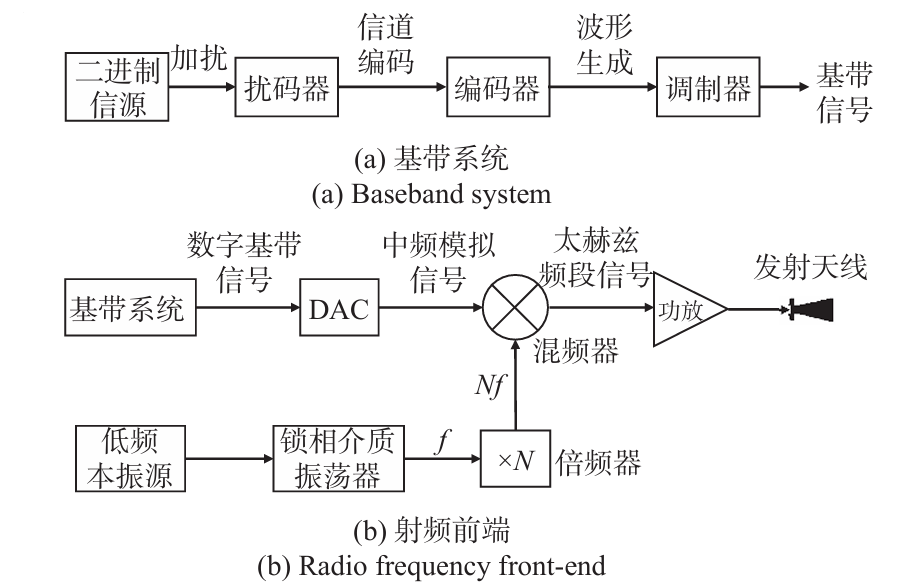
\includegraphics[width=0.6\textwidth]{img/img3.png} % 图片文件名,不需要加扩展名
	\caption{基带信号与射频前端 \cite{shi2024terahertz}}
	\label{fig:example}
\end{figure}

在射频部分,低频的本振信号依次经过锁相介质振荡器和倍频器后,被搬移到高频段。随后,混频器取倍频后信号的多次谐波,将中频模拟信号混频到指定的太赫兹频段,所得太赫兹信号经过功率放大器后,最后通过天线发射出去。

全电子型发射端的电子器件体积小、集成度高, 有利于通信系统小型化;发射功率高,可实现较远距 离无线传输。但半导体设计与加工难度受限,利用 倍频器难以产生超高频率(≥1 THz)的太赫兹信 号。此外,调制解调与编译码过程也受到基带信号 处理芯片能力限制,实时传输速率难以达到 $10^{11}$  bit/s量级及以上。


\subsection{光电子型}

得益于太赫兹波段介于微波与红外波之间,凭借其近光性,可以利用光子学方法来生成频率更高,带宽更大的太赫兹信号。由此,科学家设计了光电子型(光电外差拍频型)的太赫兹通信系统。其通过光电转换来产生太赫兹信号,借助光波的超高频率与光学器件的大带宽突破了电子器件带宽受限的问题

光电式太赫兹通信系统的发射端利用飞秒激光脉冲照射半导体材料(如 GaAs 或 InGaAs),通过光电导天线或光整流效应产生太赫兹波。其接收端:用光电导探测器、热释电探测器或肖特基二极管探测器等,将太赫兹信号转换为电信号。光电式太赫兹通信系统具有高分辨率、高灵敏度等优点。但设备复杂,成本较高,通常需要额外的光学系统支持。


\subsection{光量子型}
全电子型和光子辅助型方式产生的太赫兹信号的频率基本不超过1 THz,一般需要用量子级联型(又称直接调制激光型)方式才能产生1 THz以上的太赫兹信号。在该方法中,最常用太赫兹量子级联激光器(terahertz quantum cascade laser, THz-QCL)直接进行高速调制,但该器件对工作环境要求苛刻,需要满足低温条件,极大地限制了量子级联型方式在实际太赫兹通信系统中的应用。

\subsection{总结}
光电式太赫兹通信系统:结合光学和电子技术,具有高分辨率和高灵敏度,但设备复杂且成本较高。
全电子式太赫兹通信系统:完全基于电子学技术,设备紧凑、集成度高,适合远距离传输,但半导体设计难度大。
全光子式太赫兹通信系统:完全基于光学技术,具有高带宽和高灵敏度,适合超高数据速率的应用,但设备复杂且实时性较差。
\begin{table}[htbp]
	\centering
	\caption{太赫兹通信系统分类与对比}
	\label{tab:terahertz_systems}
	\resizebox{\textwidth}{!}{ % 自动缩放到页面宽度
		\begin{tabular}{c c c c c c p{8cm}} % 也可调窄p列
			\toprule
			\textbf{系统类型} & \textbf{信号产生方式} & \textbf{下变频方式} & \textbf{传输距离} & \textbf{系统集成度} & \textbf{光纤集成程度} & \textbf{6G典型适用场景} \\
			\midrule
			全电子型 & 基于电子学 & 全电子学 & 长 & 高 & 难 & \makecell[l]{多频段融合密集网络,通感一体车联网与AD,\\无人机自组网,卫星空间通信,军事保密通信} \\
			光子辅助型 & 基于光子学 & 光电混合 & 短 & 中 & 中 & \makecell[l]{室内XR与HC,数据中心物联网,光纤融合应急网络} \\
			全光子型 & 基于光子学 & 全光子学 & 短 & 低 & 易 & \makecell[l]{近距离探测成像,片上测试与通信} \\
			\bottomrule
		\end{tabular}
	}
%	\caption{Classification and comparison for terahertz communication systems}
\end{table}
